\documentclass{article}
\usepackage[utf8]{inputenc}
\usepackage[english,ngerman]{babel}
%% ========================================================================
%%%% MISC usepackages
%% ========================================================================

%% Chemistry
\usepackage{chemfig,chemmacros}
\chemsetup{modules = all}
\chemsetup[redox]{explicit-sign = true}
\chemsetup[phases]{pos=sub}
%\chemsetup[reactions]{before-tag = {R}, tag-open = [, tag-close = ]}
  
%% Maths
\usepackage{amsmath,amssymb,amsthm,textcomp}
\DeclareMathSymbol{*}{\mathbin}{symbols}{"01}

%% Physics
\usepackage{siunitx}

%% Graphics
\usepackage{graphicx}
\usepackage{tikz}
\usepackage{rotating}
%\usepackage{subfig}

%% Tables and Lists
\usepackage{enumerate}
\usepackage{multicol}
\usepackage{geometry}
\usepackage{tabu}
\usepackage{listings}
\usepackage{tabularx}
\usepackage{rotating}

%% Structures and Style
\usepackage{pdflscape}

\usepackage{caption}
\usepackage{subcaption}
\usepackage{booktabs}
\usepackage{colortbl}

\usepackage{xcolor}
\usepackage{xfrac}
\usepackage[export]{adjustbox}[2011/08/13]

\usepackage{booktabs}
\usepackage{float}

\usepackage{fancyhdr}

%% Data plotting
\usepackage{pgfplots}
\usepackage{filecontents}

%% Citing and Settings
\usepackage[backend=biber,
style=numeric,
backref=true, 
natbib=true, %% offering natbib-compatible commands
hyperref=true, %% using hyperref-package references
sorting= none,
doi=true,
maxcitenames=10,
maxbibnames=100,
citestyle=numeric
]{biblatex}

\addbibresource{references.bib}

\usepackage[toc,automake]{glossaries}
\include{abbrevations}
\makeglossaries

\usepackage[colorlinks=true,linkcolor=blue]{hyperref}

%% Figure settings
\renewcommand{\figurename}{Abbildung}
\renewcommand{\tablename}{Tabelle}
\renewcommand{\listfigurename}{Abbildungsverzeichnis}
\renewcommand{\listtablename}{Tabellenverzeichnis}

%% ========================================================================
%%%% Document Information
%% ========================================================================

%% Title
\title{Bestimmung der Gleichgewichtskonstante für ein Homogenes Gleichgewicht \cite{Versuchsvorschrift}} % Title
\author{Autor: Florian \textsc{Kluibenschedl}} % Author name
\date{Bericht verfasst am: \today} % Date for the report

% Page style - headers
\pagestyle{fancy}
\fancyhf{}
\rhead{PR Allgemeine Chemie A - SS2019}
\lhead{Institut für Allgemeine Chemie - Universität Innsbruck}
\rfoot{Experiment 4 - Seite \thepage}


\begin{document}
  \renewtagform{reaction}[Rgl. ]{}{}
  
  \maketitle % Insert the title, author and date
  
  \begin{center}
    \begin{tabular}{r p{4cm}}
      Versuchsdurchführung am: & 11. März 2019\\ % Date the experiment was performed
      Gruppe, Matrikelnummer: & 3, 11805747 \\
      Lehrveranstaltung: & PR Allgemeine Chemie A \\
      Institut: & Allgemeine, Anorganische und Theoretische Chemie \\
      Assistent: & Ladstätter Eva % Instructor/supervisor
    \end{tabular}
  \end{center}


  \begin{abstract}
    Gleichgewichtskonstanten spielen eine bedeutende Rolle in der Chemie. Insofern ist es unumgänglich, Methoden zu ihrer Bestimmung zu kennen. 
    
    Über photometrische Messungen wurde die Gleichgewichtskonstante der Komplexbildungsreaktion von \ch{[Fe(OH2)5SCN]\pch[2]} bestimmt. Um eine statistische Aussagekraft zu bekommen, wurde eine Verdünnungsreihe erstellt. Nach einer Fehleranalyse wurden zwei Werte für die Komplexbildungskonstante erhalten. Einer errechnete sich aus der vom Gerät direkt angegebenen Konzentration des Komplexes zu $\beta_{1} = \num[separate-uncertainty]{127 \pm 30.7}$ ($s=\num{\pm 16.7},\alpha=0.05,N=3$). Der andere wurde über die vom Gerät angegebene Extinktion bestimmt und lautet $\beta_{2} = \num[separate-uncertainty]{112 \pm 27.6}$ ($s=\num{\pm 15.0},\alpha=0.05,N=3$). Ein Vergleich mit dem Literaturwert ($\beta_{Lit.} = 134$ bei $T=\SI[mode=text]{20}{\degreeCelsius}$) zeigt, dass diese Ergebnisse recht genau sind. 
  \end{abstract}
  
  \pagebreak
  
  \section{Theoretische Grundlagen}
  
    \subsection{Motivation} \label{sec:Motivation}
      
      Die Kenntnis der Gleichgewichtskonstante einer Reaktion erlaubt diverse thermodynamische Aussagen über diese Reaktion. Es ist demnach wichtig, Methoden zu kennen, wie solche Konstanten bestimmt werden können. Im Folgenden wird dementsprechend eine Komplexbildungsreaktion näher untersucht.
      
      Das orange-gelbe \ch{Fe\pch[3]\aq} Ion bildet mit farblosem \ch{SCN\mch\aq} das blutrot gefärbte Komplexion \ch{[Fe(OH2)5SCN]\pch[2]} gemäß \ref{rec:Komplexreaktion}. 

      \begin{reaction}
        [Fe(OH2)6]\pch[3] + SCN\mch\aq{} -> [Fe(OH2)5SCN]\pch[2] + H2O \label{rec:Komplexreaktion} \\
      \end{reaction}
      
      Bei \ch{[Fe(OH2)5SCN]\pch[2]} handelt es sich um einen Charge-Transfer sowie High-Spin Komplex, was die tiefrote Farbe erklärt - Absorptionsmaximum $\lambda _{max} = $ \SI[mode=text]{485}{\nano\meter} \cite[S. 540]{InorganicChemistry}. Die Intensität der Farbe korreliert mit der Konzentration, weswegen sich die Vis-Photometrie zur Konzentrationsbestimmung eignet \cite[S. 108]{TaschenatlasAnallytik}. Sind die Konzentrationen aller Spezies in \ref{rec:Komplexreaktion} bekannt, errechnet sich nach \eqref{eq:Beta} die entsprechende Komplexbildungskonstante $\beta$. Die Konzentration von \ch{H2O} wird dabei als konstant angenommen.
      
      \begin{equation}
        \beta = \frac{[\ch{[Fe(OH2)5SCN]\pch[2]}]}{[[\ch{Fe(OH2)6]\pch[3]}] * [\ch{SCN\mch\aq}]} \label{eq:Beta}
      \end{equation} \\
      
      Anmerkung zur Angabe von Konstanten im Protokoll: um Probleme mit mathematischen Funktionen wie etwa dem Logarithmus bzw. der Exponentialfunktion zu vermeiden, werden alle Gleichgewichtskonstanten dimensionslos angegeben. Dazu werden alle Spezies im jeweiligen Massenwirkungsgesetz durch die Standardkonzentration ($c_{Standard} = 1 M$) dividiert.
      
    \subsection{Ziel des Experiments}
    
    Auf Basis der obigen Überlegungen ist das Ziel, eine möglichst exakte Bestimmung der Komplexbildungskonstante der beschriebenen Reaktion mithilfe von Vis-Photometrie durchzuführen. 
  
  \pagebreak
  
  \section{Experimenteller Teil}
  
    \subsection{Verwendete Materialien}
              
      \begin{table}[H]
        \centering
        \caption[Materialienliste, Quelle: Autor]{Auflistung der verwendeten Geräte und Chemikalien}
        \label{tab:Materialien}
        
        \begin{tabular}{@{}ll|ll@{}}
          \toprule
            Geräte & Hersteller & Chemikalie & bezogen von \\ \midrule
            6 \SI[mode=text]{16x160}{\milli\meter} Reagenzgläser  & DURAN & \SI[mode=text]{0.002}{M} \ch{NaSCN} Lösung & Vorrat \\
            Photometer & photoLab 6100 VIS & \SI[mode=text]{0.20}{M} \ch{Fe(NO3)3} Lösung & Vorrat \\
            \SI[mode=text,separate-uncertainty]{10.000(45)}{\milli\litre} Vollpipette & BRAND & deionisiertes Wasser & Labor \\
            \SI[mode=text,separate-uncertainty]{50.0(1)}{\milli\litre} Messzylinder & BRAND &  &  \\
            Glasküvetten \O \SI[mode=text]{1.6}{\centi\meter} &  &  &  \\ \bottomrule
        \end{tabular}
      \end{table}
    
    \subsection{Versuchsdurchführung} \label{sec:Versuch}
      
      Um die Gleichgewichtskonstante statistisch sinnvoll bestimmen zu können, wurde eine Verdünnungs- reihe erstellt. Dazu wurden 6 gereinigte Reagenzgläser jeweils unter Verwendung einer Vollpipette mit \SI[mode=text]{10}{\milli\liter} einer \SI[mode=text]{0.002}{M} \ch{NaSCN} Lösung gefüllt. In Reagenzglas 1 wurden mit einer Vollpipette \SI[mode=text]{10}{\milli\liter} einer \SI[mode=text]{0.20}{M} \ch{Fe(NO3)3} Lösung pipettiert. In diesem Reagenzglas liegt \ch{Fe\pch[3]\aq} im Überschuss vor ($[\ch{SCN\mch}] << [\ch{Fe\pch[3]\aq}]$, also $\ch{[Fe(OH2)5SCN]\pch[2]} = [\ch{SCN\mch}]_{0}$), weswegen es im Folgenden als Standard verwendet wurde. Anschließend wurden mit der Vollpipette \SI[mode=text]{10}{\milli\liter} einer \SI[mode=text]{0.20}{M} \ch{Fe(NO3)3} Lösung in einen \SI[mode=text]{50}{\milli\liter} Messzylinder pipettiert und mit deionisiertem Wasser auf \SI[mode=text]{25}{\milli\liter} aufgefüllt. Nach dem homogenisieren wurden \SI[mode=text]{10}{\milli\liter} entnommen\footnote{Vollpipette} und in Reagenzglas 2 pipettiert. Es wurden weitere \SI[mode=text]{5}{\milli\liter} vom Messzylinder entnommen und verworfen. Die verbleibenden \SI[mode=text]{10}{\milli\liter} wurden mit deionisiertem Wasser auf \SI[mode=text]{25}{\milli\liter} aufgefüllt, wovon wieder \SI[mode=text]{10}{\milli\liter} entnommen und in Reagenzglas 3 pipettiert wurden. Diese Prozedur wurde wiederholt, bis man 6 Reagenzgläser mit jeweils verschiedenen Konzentrationen an \ch{Fe\pch[3]\aq}, \ch{SCN\mch\aq} und \ch{[Fe(OH2)5SCN]\pch[2]} hatte - deutlich erkennbar an der abnehmenden Intensität der roten Färbung. \\
      
      Die Messung mit dem Vis-Photometer erfolgte in Glasküvetten ($d =$ \SI[mode=text]{1.6}{\centi\meter}), die ca. \SI[mode=text]{10}{\milli\liter} der Probelösung aus den Reagenzgläsern der Verdünnungsreihe enthielten. Die Probelösung wurde durch vorsichtiges Schütten in die Küvetten überführt, wobei darauf geachtet wurde, eine saubere, trockene Küvette zu verwenden, um ungewollte Konzentrationsänderungen zu vermeiden. Die Messung der Extinktion $E_{\lambda _{max}}$ erfolgte beim Absorptionsmaximum $\lambda _{max} = $ \SI[mode=text]{485}{\nano\meter}. Für die Messung wurde die Methode \textit{Eisenthiocyanat - Nr. 1001} verwendete, die bereits eine entsprechende Kalibriergerade enthält\footnote{die Bedienung des Photometers erfolgte durch den Assistenten, der auch die Hintergrundkorrektur der Grundabsorption vom Lösungsmittel \ch{H2O} durchführte}. Als Ergebnis der Messung bekam man die Konzentration von \ch{[Fe(OH2)5SCN]\pch[2]} sowie die entsprechende Extinktion $E_{\lambda _{max}}$. 
    
    \pagebreak
    
    \subsection{Auswertung}
    
      Um die Komplexbildungskonstante berechnen zu können, müssen die Gleichgewichtskonzentrationen der an der Reaktion beteiligten Spezies bekannt sein. 
      
      Bei der Verdünnungsreihe wird in jedem Schritt die Konzentration von \ch{SCN\mch}  halbiert, da das Volumen durch die Zugabe von jeweils \SI[mode=text]{10}{\milli\liter} der verdünnten \ch{Fe(NO3)3} verdoppelt wird ($V_{2} =$ \SI[mode=text]{20}{\milli\liter}). Für die \ch{Fe\pch[3]\aq} Konzentration in den Reagenzgläsern ergibt sich eine Folge, wie in \eqref{eq:FolgeKonzentrationen} dargestellt. Die genannten Konzentrationen entsprechen den Anfangskonzentrationen und sind in Tabelle \ref{tab:Messdateneins} aufgelistet. 
    
      \begin{equation}
        [\ch{Fe\pch[3]\aq}]_{n+1} = \frac{V_{n}}{V_{n+1}} * [\ch{Fe\pch[3]\aq}]_{n} = \frac{10}{25} * [\ch{Fe\pch[3]\aq}]_{n} = 0.4 * [\ch{Fe\pch[3]\aq}]_{n}\label{eq:FolgeKonzentrationen}
      \end{equation}
    
      Die Gleichgewichtskonzentrationen lassen sich wie in \eqref{eq:GGeins} und \eqref{eq:GGzwei} angeführt berechnen. Die Konzentration von \ch{[Fe(OH2)5SCN]\pch[2]} im Gleichgewicht ($[\ch{[Fe(OH2)5SCN]\pch[2]}]_{eq.}$) wurde mit dem Vis Photometer bestimmt.
      
      \begin{equation}
        [\ch{Fe\pch[3]\aq}]_{eq.} = [\ch{Fe\pch[3]\aq}]_{0} - [\ch{[Fe(OH2)5SCN]\pch[2]}]_{eq.} \label{eq:GGeins}
      \end{equation}
      
      \begin{equation}
        [\ch{SCN\mch\aq}]_{eq.} = [\ch{SCN\mch\aq}]_{0} - [\ch{[Fe(OH2)5SCN]\pch[2]}]_{eq.} \label{eq:GGzwei}
      \end{equation}
      
      Durch Einsetzen dieser Gleichgewichtskonzentration in \eqref{eq:Beta} errechnet sich die gesuchte Komplexbildungskonstante. Die theoretischen Gleichgewichtskonzentrationen von \ch{[Fe(OH2)5SCN]\pch[2]} lassen sich ausgehend von der gemessenen Extinktion, dem bekannten molaren Extinktionskoefizienten $\varepsilon_{\lambda_{max}} =$ \SI[mode=text]{4250}{\liter\per\mole\per\centi\meter} und der Schichtdicke $d =$ \SI[mode=text]{1.6}{\centi\meter} mit dem Lambert-Beer'schen Gesetz berechnen:
      
      \begin{equation}
        [\ch{[Fe(OH2)5SCN]\pch[2]}]_{theoret., eq.} = \frac{E_{\lambda_{max}}}{\varepsilon_{\lambda_{max}} * d} \label{eq:theor}
      \end{equation}
      
      Mit dieser Konzentration kann analog zu oben die Komplexbildungskonstante berechnet werden. Die beiden erhaltenen Konstanten können hinsichtlich Genauigkeit miteinander verglichen werden.
      
    \subsection{Messdaten} \label{sec:Messdaten}
    
      In den Tabellen \ref{tab:Messdatenzwei} und \ref{tab:Messdatendrei} sind alle Messwerte angeführt, die im Rahmen der Versuchsdurchführung wie in \ref{sec:Versuch} beschrieben, gemessen wurden. Tabelle \ref{tab:Messdateneins} enthält die Konzentrationen der Verdünnungsreihe.
      
      \begin{table}[H]
        \centering
        \caption[Ausgangs- und Anfangskonzentrationen, Quelle: Autor]{Ausgangs- und Anfangskonzentrationen}
        \label{tab:Messdateneins}
          \begin{tabular}{@{}llll|lll@{}}
            \toprule
             Nr. & $V_{1}$ in ml & [\ch{SCN\mch\aq}] in M & [\ch{Fe\pch[3]\aq}] in M & $V_{2}$ in ml & $[\ch{SCN\mch\aq}]_{0}$ in M & $[\ch{Fe\pch[3]\aq}]_{0}$ in M \\ \midrule
             1 & 10 & 0.002 & 0.2 & 20 & 0.001 & 0.10 \\
             2 & 10 & 0.002 & 0.08 & 20 & 0.001 & 0.040 \\
             3 & 10 & 0.002 & 0.03 & 20 & 0.001 & 0.016 \\
             4 & 10 & 0.002 & 0.01 & 20 & 0.001 & 0.0064 \\
             5 & 10 & 0.002 & 0.005 & 20 & 0.001 & 0.0026 \\
             6 & 10 & 0.002 & 0.002 & 20 & 0.001 & 0.0010 \\ \bottomrule
          \end{tabular}
      \end{table}
      
      \begin{table}[H]
        \centering
        \caption[Messergebnisse und Komplexbildungskonstanten 1, Quelle: Autor]{Messergebnisse und Komplexbildungskonstanten - Konzentrationen in \si{\mole\per\liter}}
        \label{tab:Messdatenzwei}
          \begin{tabular}{@{}lllll@{}}
            \toprule
             Nr. & $[\ch{Fe\pch[3]}]_{eq.}$ & $[\ch{SCN\mch}]_{eq.}$ & $[\ch{[Fe(OH2)5SCN]\pch[2]}]_{eq.}$ & $\beta_{1}$ \\ \midrule
             1 & \num{9.90d-2} & \num{2.80d-5} & \num{9.72e-4} & 351 \\
             2 & \num{3.90d-2} & \num{2.80d-5} & \num{9.72e-4} & 890 \\
             3 & \num{1.51d-2} & \num{1.48d-4} & \num{8.52e-4} & 381 \\
             4 & \num{5.94d-3} & \num{5.37d-4} & \num{4.63e-4} & 145 \\
             5 & \num{2.34d-3} & \num{7.75d-4} & \num{2.25e-4} & 124 \\
             6 & \num{9.30d-4} & \num{9.06d-4} & \num{9.40e-5} & 112 \\ \bottomrule
          \end{tabular}
       \end{table}  
       
       \begin{table}[H]
        \centering
        \caption[Messergebnisse und Komplexbildungskonstanten 2, Quelle: Autor]{Messergebnisse und Komplexbildungskonstanten - Konzentrationen in \si{\mole\per\liter}}
        \label{tab:Messdatendrei}
          \begin{tabular}{@{}llllll@{}}
            \toprule
             Nr. & $E_{\lambda_{max}}$ & $[\ch{[Fe(OH2)5SCN]\pch[2]}]_{th., eq.}$ & $[\ch{Fe\pch[3]}]_{eq.}$ & $[\ch{SCN\mch}]_{eq.}$ & $\beta_{2}$ \\ \midrule
             1 & 4.5 & \num{6.62e-4} & \num{9.93d-2} & \num{3.38d-4} & 19.7 \\
             2 & 4.5 & \num{6.62e-4} & \num{3.93d-2} & \num{3.38d-4} & 49.8 \\
             3 & 4.281 & \num{6.30e-4} & \num{1.54d-2} & \num{3.70d-4} & 111 \\
             4 & 2.871 & \num{4.22e-4} & \num{5.58d-3} & \num{5.78d-4} & 122 \\
             5 & 1.491 & \num{2.19e-4} & \num{2.34d-3} & \num{7.81d-4} & 120 \\
             6 & 0.559 & \num{8.22e-5} & \num{9.42d-3} & \num{9.18d-4} & 95.1 \\ \bottomrule
          \end{tabular}
       \end{table}     
       
  \pagebreak
  
  \section{Ergebnisse und Diskussion}
    
    Wird die Komplexbildungskonstante aus der gemessenen Konzentration von \ch{[Fe(OH2)5SCN]\pch[2]} berechnet, ergibt sich folgender Wert: $\beta_{1} = \num[separate-uncertainty]{334 \pm 297}$ ($s=\num{\pm 297},\alpha=0.05,N=6$). Der Ausreißertest nach Grubbs liefert, dass bei Messung 2 ein Ausreißer vorliegt. Der ausreißerbereinigte Wert für die Komplexbildungskonstante lautet nun: $\beta_{1} = \num[separate-uncertainty]{223 \pm 132}$ ($s=\num{\pm 132},\alpha=0.05,N=5$). 
    
    Wird die Komplexbildungskonstante aus der gemessenen Extinktion berechnet, ergibt sich folgender Wert: $\beta_{2} = \num[separate-uncertainty]{86.3 \pm 42.1}$ ($s=\num{\pm 42.1},\alpha=0.05,N=6$). Ein Ausreißertest nach Grubbs liefert für diesen Datensatz keinen Ausreißer.
    
    Beide, auf unterschiedliche Weise berechneten Komplexbildungsbildungskonstanten weichen recht stark vom Literaturwert ab ($\beta_{Lit.} = 134$ bei $T=\SI[mode=text]{20}{\degreeCelsius}$)\footnote{die Temperatur im Labor zum Zeitpunkt der Messungen betrug in etwa \SI[mode=text]{22}{\degreeCelsius}, weswegen der Effekt der Temperatur auf den Vergleich als vernachlässigbar erachtet wird}. Aufgrund der geringen Präzision der Messung\footnote{große Standardabweichungen} liegt der Literaturwert aber in der Verteilung beider berechneten, experimentellen Werte ($\alpha=0.05$). Für diese Abweichungen werden im Folgenden Erklärungen gesucht.\\
    
    Grundsätzlich können bei der Reaktion von \ch{Fe\pch[3]\aq} mit \ch{SCN\mch\aq} mehrere Komplexe entstehen. So sind beispielsweise die Komplexe \ch{[Fe(OH2)4SCN2]\pch} oder \ch{[Fe(OH2)3SCN3]} denkbar. Welcher Komplex nun tatsächlich entsteht, hängt von den Bedingungen ab. Bei den in diesem Versuch gegebenen Bedingungen ist  die Bildung von \ch{[Fe(OH2)5SCN]\pch[2]} am wahrscheinlichsten, da eine \ch{SCN\mch\aq} Lösung mit geringer Konzentration verwendet wurde \cite[S. 125]{Wasseranalyse}. Die Entstehung anderer Komplexe kann demnach tatsächlich vernachlässigt werden. Da wie in \cite[S. 125]{Wasseranalyse} beschrieben, der \pH-Wert auf die Reaktion einen großen Einfluss hat, dieser jedoch nicht bestimmt wurde bzw. nicht bekannt ist, könnte dies eine Fehlerquelle sein. Wie oben beschrieben, werden deutlich unterschiedliche Werte für die Komplexbildungskonstante bei unterschiedlicher Auswertung erhalten. Dies unterstützt die Vermutung, dass die Kalibrierung des Messgerätes bzw. dessen Einstellungen fehlerbehaftet sind. Eine weitere Fehlerquelle liegt natürlich in der Herstellung der Verdünnungsreihe. \\
    
    Wie aus den Messdaten in \ref{sec:Messdaten} abgelesen werden kann, weichen die ersten drei Messwerte bei beiden Berechnungsmethoden am stärksten vom Literaturwert ab. Dies lässt sich durch die hohe Konzentration an \ch{[Fe(OH2)5SCN]\pch[2]} und \ch{Fe\pch[3]\aq} erklären. Da \ch{Fe\pch[3]\aq} bei $\lambda = \SI[mode=text]{485}{nm}$ auch absorbiert, wird dessen Konzentration in jene von \ch{[Fe(OH2)5SCN]\pch[2]} unfreiwillig miteinbezogen. Das bedeutet, die gemessene \ch{[Fe(OH2)5SCN]\pch[2]} Konzentration und damit die Komplexbildungskonstante sind zu hoch. Bei niedrigeren \ch{Fe\pch[3]\aq} Konzentrationen ist dieser Fehler nicht so groß, weswegen die Werte der Messungen 4,5 und 6 sich dem Literaturwert für die Komplexbildungskonstante annähern. Der auf diese Weise berechnete Wert aus den Daten von Tabelle \ref{tab:Messdatenzwei} lautet $\beta_{1} = \num[separate-uncertainty]{127 \pm 30.7}$ ($s=\num{\pm 16.7},\alpha=0.05,N=3$) und kommt dem Literaturwert schon sehr nahe. Wird der Wert aus den Daten von Tabelle \ref{tab:Messdatendrei} (aus der gemessenen Extinktion) berechnet, ergibt sich $\beta_{2} = \num[separate-uncertainty]{112 \pm 27.6}$ ($s=\num{\pm 15.0},\alpha=0.05,N=3$). Zu beachten ist, dass bei diesen Werten auch die Präzision in einem annehmbaren Rahmen liegt.
    
    Dass die Messungen bei höheren Konzentrationen nicht berücksichtigt werden müssen, geht auch aus den Graphen in Abbildung \ref{fig:Extinktion} und \ref{fig:Konzentration} hervor. Bei geringen Konzentrationen kommen die Messwerte den Werten des linearen Modells, das mithilfe des Lambert-Beerschen Gesetzes berechnet wurde, sehr nahe. Bei größeren Konzentrationen nimmt die Abweichung zu.
    
    \subsubsection{Auswertung der Abweichungen bei unterschiedlichen Konzentrationen}
    
    \begin{figure}[H]
      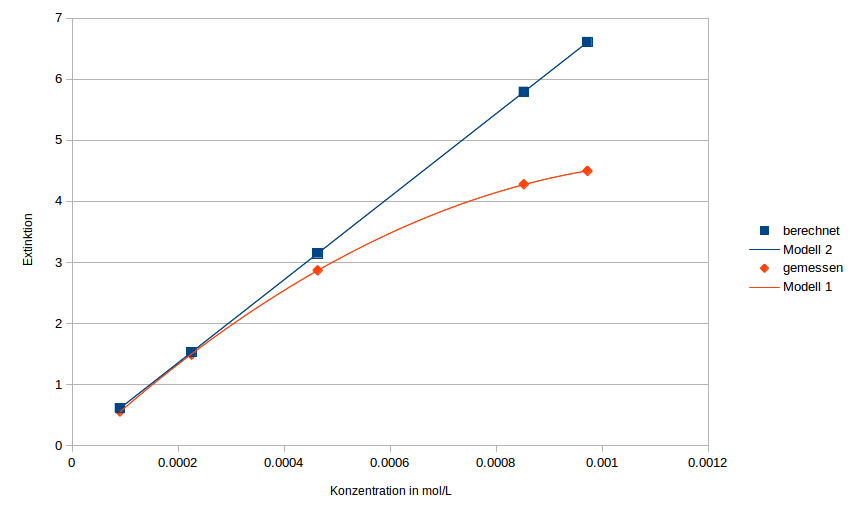
\includegraphics[scale=0.7, center]{Graphiken/Ergebnisse/ExtinktiongegenKonzentration.png} 
      \caption[Graph Auftragung der Extinktion gegen die Konzentration, Quelle: Autor]{Auftragung der Extinktion gegen die Konzentration von $\ch{[Fe(OH2)5SCN]\pch[2]}_{eq.}$: \\ Modell 2 $=6800 x-\num{7.25d-16}, R^2=1$; Modell 1 $=\num{-3.40d6} x^2 + \num{8.09d3} x - 0.147, R^2 \approx 1$}
      \label{fig:Extinktion}
    \end{figure}
    
    \begin{figure}[H]
      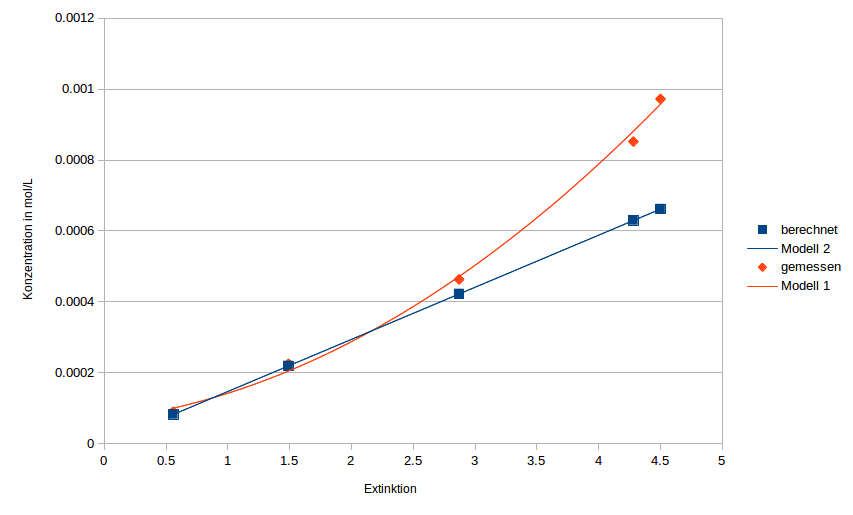
\includegraphics[scale=0.7, center]{Graphiken/Ergebnisse/KonzentrationgegenExtinktion.png} 
      \caption[Graph Auftragung der Konzentration gegen die Extinktion, Quelle: Autor]{Auftragung der Konzentration gegen die Extinktion von $\ch{[Fe(OH2)5SCN]\pch[2]}_{eq.}$: \\ Modell 2 $=\num{1.47d-4} x, R^2=1$; Modell 1 $=\num{3.50d-5} x^2 + \num{4.06d-5} x - \num{6.65d-5}, R^2 = 0.998$}
      \label{fig:Konzentration}
    \end{figure}
    
  \pagebreak
  
  \listofreactions
  \printbibliography[title=Literaturverzeichnis]
  \listoffigures
  \listoftables
  
\end{document}
